\chapter{Project Framework and Methodology}\label{chap:project}
\fancyhead[R]{Project Framework and Methodology}

\textit{``This chapter establishes the comprehensive project framework for developing the real-time fee calculation system within the P2S financial platform. It covers the project context, host organization, problem definition, solution approach, project management methodology, and technical foundations that guide the implementation of stateless computational engines.''}

\pagebreak

\section{Introduction}

The development of high-performance fee calculation systems represents a critical challenge for financial institutions operating within the French electronic payment ecosystem. This project addresses fundamental inefficiencies in contemporary payment processing through the design and implementation of stateless computational engines optimized for real-time transaction fee determination.

The project operates within the Payment Steering Solution (P2S) initiative, focusing specifically on the development of scalable computational architectures that leverage pre-normalized fee structures to achieve optimal performance characteristics. The primary objective is creating a robust framework capable of processing high-volume transaction streams while maintaining accuracy and compliance with payment scheme regulations.

This chapter establishes the foundational framework for the project, including organizational context, problem definition, solution methodology, and management approach that guides the subsequent technical development phases.

\section{Project Context and Motivation}

The French electronic payment ecosystem operates within a complex regulatory framework involving multiple stakeholders including issuing banks, acquiring banks, payment schemes, and regulatory authorities. Financial institutions must navigate intricate fee schedules, interchange rates, and processing charges that vary significantly based on transaction type, merchant category, geographic location, and numerous other parameters.

\subsection{Current Challenges in Fee Processing}

The calculation and validation of transaction fees present significant operational challenges that manifest in two primary domains:

\textbf{Structural Complexity:} Payment schemes distribute fee specifications through inconsistent documentation formats, predominantly as unstructured PDF documents exceeding several hundred pages. These documents contain embedded tabular data, conditional logic expressed in natural language, and complex cross-references that resist systematic computational interpretation without prior normalization.

\textbf{Computational Limitations:} Traditional fee calculation systems rely on monolithic architectures with hard-coded logic, resulting in several critical limitations:

\begin{itemize}
   \item \textbf{Performance Degradation:} Processing throughput exhibits inverse correlation with rule complexity, creating bottlenecks in high-volume environments
   \item \textbf{Maintenance Overhead:} Manual interpretation and hard-coding of fee rules creates maintenance complexity that scales poorly with specification update frequency
   \item \textbf{Scalability Constraints:} Monolithic frameworks lack the modularity necessary for dynamic scaling and efficient resource utilization
   \item \textbf{Processing Inflexibility:} Existing systems cannot efficiently leverage normalized data structures when available
\end{itemize}

\subsection{Business Impact}

These limitations result in measurable business impacts for financial institutions:

\begin{itemize}
   \item Increased operational costs due to manual fee validation processes
   \item Reduced transaction processing capacity during peak periods
   \item Higher risk of fee calculation errors and compliance issues
   \item Limited ability to adapt quickly to new payment scheme requirements
   \item Suboptimal resource utilization requiring over-provisioning of computational infrastructure
\end{itemize}

\subsection{Solution Approach}

This project addresses these challenges through an integrated framework comprising two complementary components:

\textbf{Normalization Framework:} Transforms heterogeneous payment scheme documentation into standardized, computationally-optimized data structures while preserving the semantic integrity of fee determination logic.

\textbf{Stateless Computational Architecture:} Leverages normalized data structures through dedicated, high-performance processing engines designed for optimal fee determination in real-time environments.

The architectural integration between these components enables horizontal scalability, fault isolation, and optimized resource utilization while eliminating real-time parsing overhead during transaction processing.

\section{Presentation of the Host Organization}

Effyis Group is a management and technology consulting firm founded in 2015 and headquartered in Paris, France. The company operates as a SARL (Limited Liability Company) with a capital of 150,000€ and reported revenue of 8.8M€ in 2020. With approximately 150 employees across two continents, Effyis positions itself as a medium-sized enterprise specializing in digital transformation for financial services.

\subsection{Organizational Structure}

Effyis Group operates with a flat organizational structure that minimizes management layers between executives and staff. This approach enables faster decision-making, more direct communication, and greater employee autonomy. Teams are formed dynamically based on project requirements, duration, and complexity rather than rigid hierarchical structures.

\subsection{Business Divisions}

The company operates through four main business divisions:

\begin{itemize}
    \item \textbf{Consulting:} Strategic planning, implementation assistance, and change management services for organizational transformation projects
    \item \textbf{Digital Factory:} Web and mobile application development using agile methodologies and customer-centered design approaches
    \item \textbf{Data Lab:} Data analytics services including strategy development, data science, governance frameworks, and visualization solutions
    \item \textbf{Payment:} Payment systems implementation, integration, platform certification, and regulatory compliance services
\end{itemize}

\subsection{Industry Specialization}

Effyis Group focuses on several key sectors:

\begin{itemize}
    \item \textbf{Banking:} Comprehensive services covering retail, corporate, private, and investment banking operations
    \item \textbf{Payment:} Support for banks, payment institutions, fintech companies, and startups in developing innovative payment solutions
    \item \textbf{Industry:} Operational optimization for pharmaceutical, automotive, telecommunications, and transportation companies
    \item \textbf{Insurance:} Digital transformation support through strategic planning, organizational restructuring, and innovation projects
\end{itemize}

\subsection{Key Products}

Effyis Group has developed several proprietary solutions:

\begin{itemize}
    \item \textbf{Lodin:} An open banking platform providing AISP and PISP functionalities for secure financial data exchange and payment processing
    \item \textbf{Payment Steering Solution (P2S):} A payment processing optimization system that analyzes and predicts interchange and scheme fees for financial institutions, including comprehensive billing management capabilities
\end{itemize}

\subsection{Company Profile}

\begin{table}[ht]
    \centering
    \begin{tabular}{|l|l|}
        \hline
        \textbf{Attribute} & \textbf{Details} \\
        \hline
        Company Name & EFFYIS Group \\
        \hline
        Founded & 2015 \\
        \hline
        Legal Structure & SARL (Société à Responsabilité Limitée) \\
        \hline
        Business Focus & Management and Technology Consulting \\
        \hline
        Company Size & 150 employees across 2 continents \\
        \hline
        Headquarters & 140 bis rue de Rennes 75006, PARIS \\
        \hline
        Capital & 150,000€ \\
        \hline
        Annual Revenue & 8.8M€ (2020) \\
        \hline
    \end{tabular}
    \caption{EFFYIS Group Company Information}
\end{table}


\section{Problem Statement}

This project addresses a fundamental inefficiency in contemporary payment processing systems that manifests through two interconnected challenges affecting the French financial infrastructure.

\subsection{Primary Problem}

Financial institutions face significant operational inefficiencies when processing transaction fees from international payment networks due to:

\textbf{Structural Heterogeneity:} Payment schemes distribute fee specifications through inconsistent documentation formats that resist systematic computational interpretation. These documents, typically exceeding several hundred pages, contain embedded tabular data, conditional natural language expressions, and complex cross-references that require manual interpretation and hard-coding of fee logic.

\textbf{Computational Bottlenecks:} Traditional processing architectures demonstrate exponential performance degradation as rule complexity increases. Current systems exhibit:
\begin{itemize}
   \item Processing latency that scales poorly with rule complexity
   \item Resource contention in shared processing environments
   \item Sequential rule evaluation that cannot leverage parallel processing
   \item Inability to efficiently utilize normalized data structures
\end{itemize}

\subsection{Business Impact}

These limitations result in measurable operational impacts:

\begin{itemize}
   \item \textbf{Increased Processing Costs:} Manual validation processes and over-provisioned infrastructure
   \item \textbf{Reduced Throughput:} Performance bottlenecks during peak transaction periods
   \item \textbf{Compliance Risk:} Higher probability of fee calculation errors and regulatory violations
   \item \textbf{Operational Inflexibility:} Limited ability to adapt to changing payment scheme requirements
\end{itemize}

\subsection{Technical Challenges}

The compound nature of these challenges requires a comprehensive solution addressing both structural and computational dimensions:

\begin{itemize}
   \item Transformation of heterogeneous documentation into standardized, machine-readable formats
   \item Development of high-performance computational engines optimized for normalized rule application
   \item Implementation of scalable architecture supporting real-time processing requirements
   \item Integration with existing payment processing infrastructure
\end{itemize}

\section{Project Scope}

This project focuses on the design, implementation, and validation of a \textbf{proof-of-concept stateless computational architecture} for real-time fee calculation within the P2S platform. The work serves as a foundation for the broader P2S production system that will be developed in subsequent phases beyond this internship period.

\subsection{Project Framework Context}

The complete P2S framework envisioned consists of two interconnected components:

\subsubsection{Rule Normalization Framework}
Systematic transformation of heterogeneous payment scheme documentation into standardized, computationally-optimized data formats while preserving semantic integrity of fee determination logic. \textit{(Future production development - out of scope for this internship)}

\subsubsection{Stateless Computational Engine Architecture}
High-performance processing engines operating on normalized data structures to achieve optimal fee determination in real-time environments. \textbf{This component represents the primary focus of this internship project as a proof-of-concept implementation.}

\subsection{Internship Project Focus}

This internship project concentrates specifically on developing and validating the core concepts of the stateless computational engine architecture through:

\begin{enumerate}
    \item \textbf{Proof-of-Concept Architecture:} Development of foundational computational engine components demonstrating the viability of the stateless approach
    \item \textbf{Core Algorithm Implementation:} Implementation of essential transaction processing and fee calculation logic with basic optimization
    \item \textbf{Performance Baseline Validation:} Establishing performance baselines and demonstrating scalability potential for future production deployment
    \item \textbf{Integration Foundation:} Creating the integration framework and messaging patterns for future production enhancement
\end{enumerate}

\subsection{Project Boundaries}

\textbf{In Scope (Proof-of-Concept Deliverables):}
\begin{itemize}
    \item Core stateless computational engine architecture design and basic implementation
    \item Foundational transaction processing pipeline with essential optimization
    \item Basic integration with P2S platform components and messaging infrastructure
    \item Performance baseline establishment and scalability concept validation
    \item Support for key DMS processing patterns
    \item Development environment deployment and testing framework
\end{itemize}

\textbf{Out of Scope (Reserved for Future Production Development):}
\begin{itemize}
    \item Production-scale deployment and full operational optimization
    \item Complete fee rule extraction and automatic data normalization
    \item Comprehensive international payment network coverage
    \item Advanced performance tuning and enterprise-grade monitoring
    \item Full regulatory compliance framework implementation
    \item Complete P2S platform integration and production deployment
\end{itemize}

\subsection{Project Constraints and Key Assumptions}

\textbf{Data Model Constraints:}
The implementation operates under the assumption of evolving input data schemas, requiring flexible architecture to accommodate ongoing specification changes from the client organization.

\textbf{Infrastructure Constraints:}
Development and testing conducted on shared development infrastructure, with production performance projections based on architectural analysis rather than dedicated environment testing.

\section{Project Charter}

The project charter establishes the foundational framework for developing the real-time fee calculation system within the P2S financial platform.

\subsection{Project Objectives}

\begin{itemize}
    \item \textbf{Proof-of-Concept Validation:} Develop and validate the fundamental concepts of stateless computational architecture for fee calculation with processing capabilities demonstrating scalability potential
    \item \textbf{Foundation Integration:} Establish basic integration patterns with P2S infrastructure and messaging components, creating the foundation for future production deployment
    \item \textbf{Architecture Demonstration:} Demonstrate the viability of event-driven, stateless processing architecture through working prototype implementation
    \item \textbf{Performance Baseline:} Establish performance baselines (target: 1000+ TPS) and validate horizontal scaling concepts through development environment testing
\end{itemize}

\subsection{Project Deliverables}

\begin{itemize}
    \item \textbf{Proof-of-Concept Computational Framework:} Foundational fee calculation engines demonstrating stateless architecture viability and basic microservices patterns
    \item \textbf{Basic Integration Components:} Essential message broker integration, basic caching implementation, and database connectivity foundation
    \item \textbf{Core Validation Framework:} Fundamental data validation with ISO 20022-inspired structure and essential business rule verification
    \item \textbf{Technical Documentation:} Architecture design documentation, implementation guidelines, and performance analysis for future production development
    \item \textbf{Development Testing Suite:} Core testing framework with unit tests, basic integration tests, and performance baseline validation tools
\end{itemize}

\section{Project Requirements}

\subsection{Functional Requirements}

\subsubsection{Core Processing Capabilities}
\begin{itemize}
    \item \textbf{Data Validation:} Financial message structure validation based on ISO 20022 principles and business rule verification
    \item \textbf{Context Analysis:} Geographic classification, merchant categorization, and payment instrument identification
    \item \textbf{Fee Computation:} Interchange and scheme fee calculation with support for multiple determination methods
    \item \textbf{System Integration:} Kafka message processing, database operations, and caching integration
\end{itemize}

\subsection{Non-Functional Requirements}

\subsubsection{Performance Characteristics}
\begin{itemize}
    \item \textbf{Processing Efficiency:} Concurrent transaction processing through stateless architecture
    \item \textbf{Response Time:} Sub-second processing latency for real-time operations
    \item \textbf{Resource Optimization:} Efficient memory and CPU utilization with intelligent caching
\end{itemize}

\subsubsection{Quality Attributes}
\begin{itemize}
    \item \textbf{Accuracy:} Consistent fee calculations aligned with payment scheme specifications
    \item \textbf{Reliability:} Graceful error handling and recovery mechanisms
    \item \textbf{Maintainability:} Modular architecture supporting independent component development
    \item \textbf{Security:} Compliance with financial industry security standards and audit requirements
\end{itemize}
\section{Project Management}

This section outlines the project management approach and development methodology employed throughout the development of the real-time fee calculation system within the P2S financial platform. The project adopted the Agile Scrum framework to ensure iterative development, continuous stakeholder engagement, and adaptive planning in response to the complex requirements of financial transaction processing.

\subsection{Project Conduct}

The project conduct was structured around collaborative development principles, emphasizing transparent communication between all stakeholders. Regular coordination meetings were established to ensure alignment between technical development activities and business objectives. The conduct framework incorporated continuous feedback loops with the client, enabling rapid adaptation to evolving requirements while maintaining focus on the core objectives of real-time fee calculation optimization.

The project execution followed established professional practices within Effyis Group, ensuring compliance with organizational standards for quality, security, and documentation. Weekly progress reviews were conducted with the product owner to validate deliverables against business requirements and adjust priorities based on emerging technical insights.

\subsection{Project Methodology}

The project methodology was designed to address the inherent complexity of financial transaction processing while maintaining flexibility for iterative improvement. The methodology encompassed several key principles:

\textbf{Iterative Development Approach:} Complex system components were developed incrementally, allowing for early validation of architectural decisions and performance characteristics. This approach proved particularly valuable for the stateless worker engine development, where performance optimization required multiple refinement cycles.

\textbf{Continuous Integration and Validation:} Each development increment was integrated into the broader system architecture and validated against functional and performance requirements. This approach enabled early detection of integration issues and performance bottlenecks.

\textbf{Risk-Driven Development:} Technical risks, particularly those related to real-time processing requirements and system scalability, were addressed early in the development cycle through proof-of-concept implementations and performance testing.

\textbf{Stakeholder-Centric Design:} Regular stakeholder engagement ensured that the system design remained aligned with operational requirements and business objectives throughout the development process.

\subsection{Why Scrum}

The selection of Scrum as the primary project management framework was driven by several factors specific to the nature of financial transaction processing system development:

\textbf{Complexity Management:} The intricate nature of fee calculation algorithms and their integration with existing P2S platform components required an iterative approach that could accommodate complexity without compromising system integrity. Scrum's structured approach to managing complex product development aligned well with these requirements.

\textbf{Stakeholder Engagement:} Financial institutions require high levels of transparency and validation throughout system development. Scrum's emphasis on regular stakeholder demonstration and feedback facilitated continuous alignment with business requirements and enabled rapid adjustment to evolving needs.

\textbf{Risk Mitigation:} The high-stakes nature of financial transaction processing demanded early identification and mitigation of technical risks. Scrum's sprint-based approach enabled regular risk assessment and adjustment of development priorities based on emerging technical insights.

\textbf{Team Collaboration:} The multidisciplinary nature of the development team, including backend developers, data scientists, and DevOps engineers, required a framework that facilitated effective collaboration. Scrum's emphasis on cross-functional team collaboration and regular communication proved essential for coordinating the diverse technical contributions required for system success.

\textbf{Adaptability:} The evolving understanding of performance optimization requirements and integration complexities necessitated an adaptive development approach. Scrum's flexibility in adjusting priorities and scope based on learning and feedback provided the necessary adaptability for successful system development.

\subsection{Team Structure and Roles}

The project team structure was organized according to Scrum roles while accommodating the specialized requirements of financial system development:

\subsubsection{Core Scrum Roles}

\textbf{Product Owner - Mr. Zakaria ZAZA:} Represented the P2S platform stakeholders, defining and prioritizing business requirements. Responsibilities included facilitating client meetings, validating system functionality against business objectives, and ensuring alignment between technical development and operational transparency goals. The Product Owner maintained the product backlog and made critical decisions regarding feature prioritization and acceptance criteria.

\textbf{Scrum Master - Mr. Abdelkhalek ABRIL:} Served as both internship supervisor and Scrum Master, facilitating sprint ceremonies and removing development impediments. Provided technical guidance on financial payment processing standards while ensuring adherence to Scrum principles. Responsibilities included coaching the team on Scrum practices, facilitating communication between team members, and ensuring continuous improvement of development processes.

\textbf{Development Team:} Cross-functional team responsible for delivering system functionality within sprint commitments.

\subsubsection{Specialized Technical Roles}

\textbf{Backend Development Team:}

Mr. Anas TAHA and Mr. Nasserallah ELMASSAOUDI: Responsible for implementing stateless worker services, designing cost code mechanisms, and integrating with event-driven architecture. Collaborated on system-wide integration tasks and performance optimization initiatives.

\textbf{Data Science Team:}

Mr. Khalil HAMDAOUI and Mr. Ahmed Amine BELAROUSSIA: Focused on normalization of payment scheme documentation, ensuring structured rule sets were available for computational engines. Collaborated with backend developers to optimize rule application algorithms.

\textbf{DevOps Team:}

Mr. Khalil HARIR and Mr. Soufiane: Responsible for deployment pipeline management, containerization of stateless worker services, cloud infrastructure deployment, and continuous monitoring implementation. Integrated SAST and DAST security scanning tools into the deployment process.

\subsubsection{Team Collaboration Framework}

The team operated under a collaborative framework that emphasized knowledge sharing and cross-functional cooperation. Regular technical discussions were conducted to ensure alignment between different technical domains and to address integration challenges proactively.

\subsection{Project Schedule and Timeline}

The implementation of the Scrum agile methodology for this project was executed over a four-month period (February 28, 2025 - June 1, 2025), with each phase carefully planned to address the complexities of payment processing fee computation. The project timeline illustrates the allocation of resources and the overlapping nature of certain phases, characteristic of Scrum agile's iterative approach.

\begin{figure}[H]
    \centering
    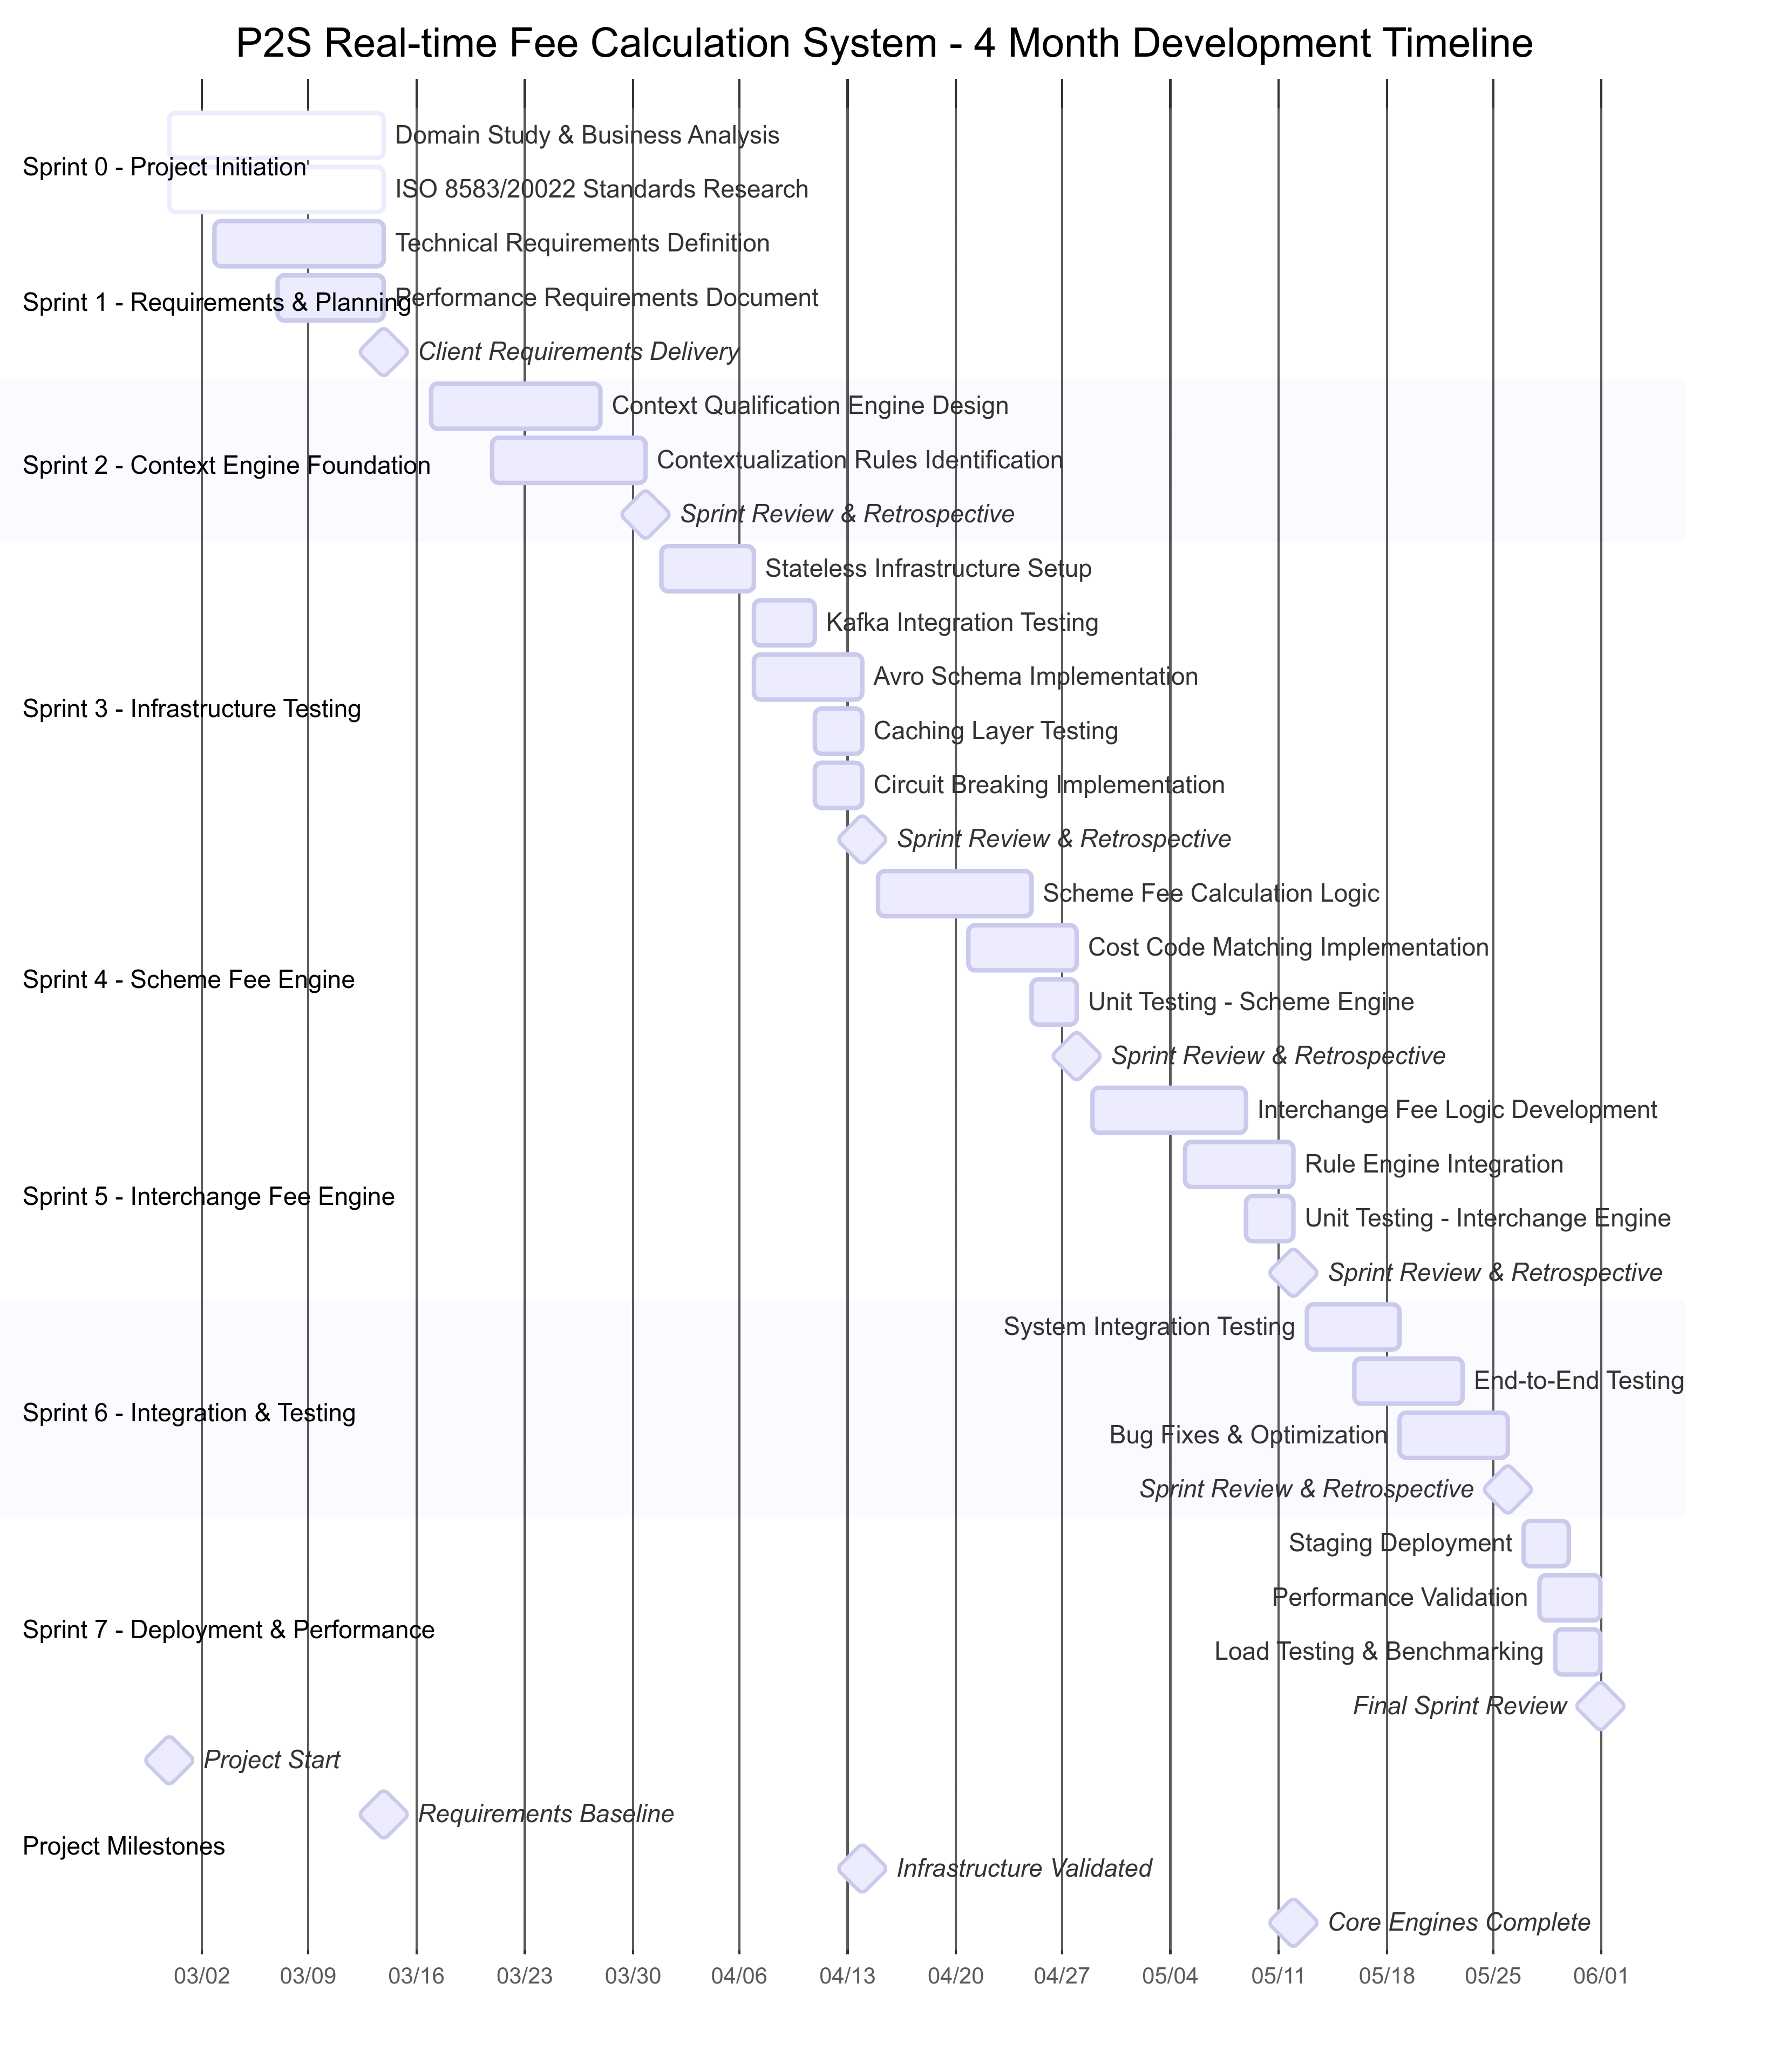
\includegraphics[width=\textwidth]{img/gantt.png}
    \caption{Project Timeline - Gantt Diagram}
    \label{fig:gantt}
\end{figure}

\subsubsection{Sprint Structure and Ceremonies}

\textbf{Sprint Planning:} Two-week sprints were established to provide sufficient time for complex development tasks while maintaining regular feedback cycles. Sprint planning sessions involved detailed technical analysis of user stories, estimation of development effort, and identification of dependencies between system components.

\textbf{Daily Standups:} Daily coordination meetings focused on progress updates, impediment identification, and coordination of interdependent development activities. These meetings proved particularly valuable for coordinating the integration of stateless worker engines with the broader P2S platform architecture.

\textbf{Sprint Reviews:} Bi-weekly demonstrations to stakeholders showcased completed functionality and gathered feedback on system behavior and performance characteristics. These sessions facilitated continuous validation of system alignment with business requirements.

\textbf{Sprint Retrospectives:} Regular reflection sessions identified process improvements and addressed technical challenges encountered during development. These sessions proved valuable for optimizing development practices and addressing emerging technical complexities.

\subsection{Product Backlog}

The product backlog was structured to reflect the actual project timeline and technical complexity of the real-time fee calculation system development:

\subsubsection{Epic-Level Organization}

\textbf{Sprint 0 - Project Initiation (Feb 28 - Mar 14):}
\begin{itemize}
    \item Domain Study \& Business Analysis of Electronic Payment Industry
    \item ISO 8583 and ISO 20022 Standards Research
    \item Market research and competitive analysis
\end{itemize}

\textbf{Sprint 1 - Requirements \& Planning (Mar 3 - Mar 14):}
\begin{itemize}
    \item Technical Requirements Definition
    \item Performance Requirements Document
    \item Client Requirements Delivery and Validation
\end{itemize}

\textbf{Sprint 2 - Context Engine Foundation (Mar 17 - Mar 31):}
\begin{itemize}
    \item Context Qualification Engine Design
    \item Contextualization Rules Identification
    \item Transaction context analysis framework
\end{itemize}

\textbf{Sprint 3 - Infrastructure Testing (Apr 1 - Apr 14):}
\begin{itemize}
    \item Stateless Infrastructure Setup
    \item Kafka Integration Testing
    \item Avro Schema Implementation
    \item Caching Layer Testing
    \item Circuit Breaking Implementation
\end{itemize}

\textbf{Sprint 4 - Scheme Fee Engine (Apr 15 - Apr 28):}
\begin{itemize}
    \item Scheme Fee Calculation Logic
    \item Cost Code Matching Implementation
    \item Unit Testing for Scheme Engine
\end{itemize}

\textbf{Sprint 5 - Interchange Fee Engine (Apr 29 - May 12):}
\begin{itemize}
    \item Interchange Fee Logic Development
    \item Rule Engine Integration
    \item Unit Testing for Interchange Engine
\end{itemize}

\textbf{Sprint 6 - Integration \& Testing (May 13 - May 26):}
\begin{itemize}
    \item System Integration Testing
    \item End-to-End Testing
    \item Bug Fixes \& Optimization
\end{itemize}

\textbf{Sprint 7 - Deployment \& Performance (May 27 - Jun 1):}
\begin{itemize}
    \item Production Deployment
    \item Performance Validation
    \item Load Testing \& Benchmarking
\end{itemize}

\subsubsection{User Story Structure}

User stories were crafted to reflect the actual development progression and business value delivery:

\textbf{Domain Understanding Phase:}
\begin{itemize}
    \item As a development team member, I want to understand the electronic payment industry standards so that I can build compliant fee calculation systems.
    \item As a developer, I want to study ISO 8583 and ISO 20022 standards so that I can implement proper message handling and processing.
\end{itemize}

\textbf{Requirements Phase:}
\begin{itemize}
    \item As a financial institution operator, I want clear technical requirements documentation so that I understand system capabilities and constraints.
    \item As a product owner, I want performance requirements defined so that I can validate system meets business needs.
\end{itemize}

\textbf{Engine Development Phase:}
\begin{itemize}
    \item As a financial institution operator, I want context qualification functionality so that I can properly categorize transactions for fee calculation.
    \item As a system user, I want scheme fee calculation so that I can determine appropriate fees based on payment scheme rules.
    \item As a financial institution, I want interchange fee calculation so that I can process inter-bank transaction fees accurately.
\end{itemize}

\textbf{Infrastructure Phase:}
\begin{itemize}
    \item As a system administrator, I want stateless infrastructure so that I can ensure system scalability and reliability.
    \item As a developer, I want Kafka integration so that I can process messages in real-time.
    \item As a system architect, I want caching and circuit breaking so that I can ensure system resilience.
\end{itemize}

\textbf{Integration Phase:}
\begin{itemize}
    \item As a system operator, I want integrated fee calculation engines so that I can process complete transaction fee calculations.
    \item As a quality assurance engineer, I want comprehensive testing so that I can validate system functionality and performance.
\end{itemize}

\subsubsection{Acceptance Criteria Framework}

Each user story included detailed acceptance criteria addressing functional requirements, performance expectations, and compliance considerations:

\begin{itemize}
    \item \textbf{Functional Criteria:} Core engine functionality, data validation, rule processing
    \item \textbf{Performance Criteria:} Response time requirements, throughput specifications, scalability metrics
    \item \textbf{Integration Criteria:} Message broker connectivity, database operations, API compatibility
    \item \textbf{Quality Criteria:} Error handling, logging, monitoring, security compliance
\end{itemize}

\subsection{Priorities}

The prioritization framework balanced business value delivery with technical risk mitigation and followed the actual project execution sequence:

\subsubsection{Priority Framework}

\begin{itemize}
    \item \textbf{Critical Priority:} Domain understanding, requirements definition, and core engine development
    \item \textbf{High Priority:} Infrastructure testing, integration components, and system validation
    \item \textbf{Medium Priority:} Performance optimization, comprehensive testing, and deployment preparation
    \item \textbf{Low Priority:} Advanced monitoring features, reporting enhancements, and system optimizations
\end{itemize}

\subsubsection{Dynamic Priority Adjustment}

Priorities were regularly reviewed and adjusted based on stakeholder feedback, technical discoveries, and emerging business requirements. The Product Owner maintained authority over priority decisions while incorporating input from technical team members regarding implementation complexity and risk factors.

\subsection{Quality Assurance and Testing Strategy}

The Agile approach incorporated continuous testing throughout the development lifecycle:

\textbf{Unit Testing:} Each engine component was thoroughly tested in isolation to ensure correct functionality and performance characteristics.

\textbf{Integration Testing:} Comprehensive testing of system components working together, particularly focusing on message broker integration and data flow validation.

\textbf{Performance Testing:} Continuous validation of system performance against real-time processing requirements, including load testing and benchmarking.

\textbf{End-to-End Testing:} Complete transaction flow testing to validate the entire fee calculation process from message receipt to result delivery.

\subsection{Risk Management}

Risk management was integrated throughout the project lifecycle, with particular attention to technical and operational risks:

\subsubsection{Technical Risks}

\begin{itemize}
    \item \textbf{Performance Degradation:} Mitigated through early performance testing and optimization
    \item \textbf{Integration Complexity:} Addressed through incremental integration and thorough testing
    \item \textbf{Data Consistency:} Managed through validation frameworks and audit trails
\end{itemize}

\subsubsection{Operational Risks}

\begin{itemize}
    \item \textbf{Resource Availability:} Mitigated through knowledge sharing and cross-training
    \item \textbf{Requirement Evolution:} Managed through regular stakeholder engagement and adaptive planning
    \item \textbf{Compliance Requirements:} Addressed through regular compliance reviews and validation
\end{itemize}

\subsection{Project Milestones}

Key milestones were established to provide checkpoints for progress evaluation:

\begin{itemize}
    \item \textbf{Project Start (Feb 28, 2025):} Project initiation and team setup
    \item \textbf{Requirements Baseline (Mar 14, 2025):} Complete requirements documentation and client approval
    \item \textbf{Infrastructure Validated (Apr 14, 2025):} Stateless infrastructure and messaging system ready
    \item \textbf{Core Engines Complete (May 12, 2025):} All fee calculation engines implemented and tested
    \item \textbf{System Integration Complete (May 26, 2025):} Full system integration and validation
    \item \textbf{Project Completion (Jun 1, 2025):} Production deployment and performance validation
\end{itemize}

This structured approach ensured successful delivery of the real-time fee calculation system while maintaining high quality standards and stakeholder satisfaction throughout the development process.

\section{System Architecture}

\subsection{Ecosystem Overview}

The Payment Steering Solution (P2S) operates within a comprehensive financial transaction processing ecosystem designed to address the computational challenges of real-time fee calculation in the French payment industry. The ecosystem encompasses multiple interconnected components that collectively enable automated processing of complex payment scheme documentation and real-time transaction fee computation.

\begin{figure}[H]
    \centering
    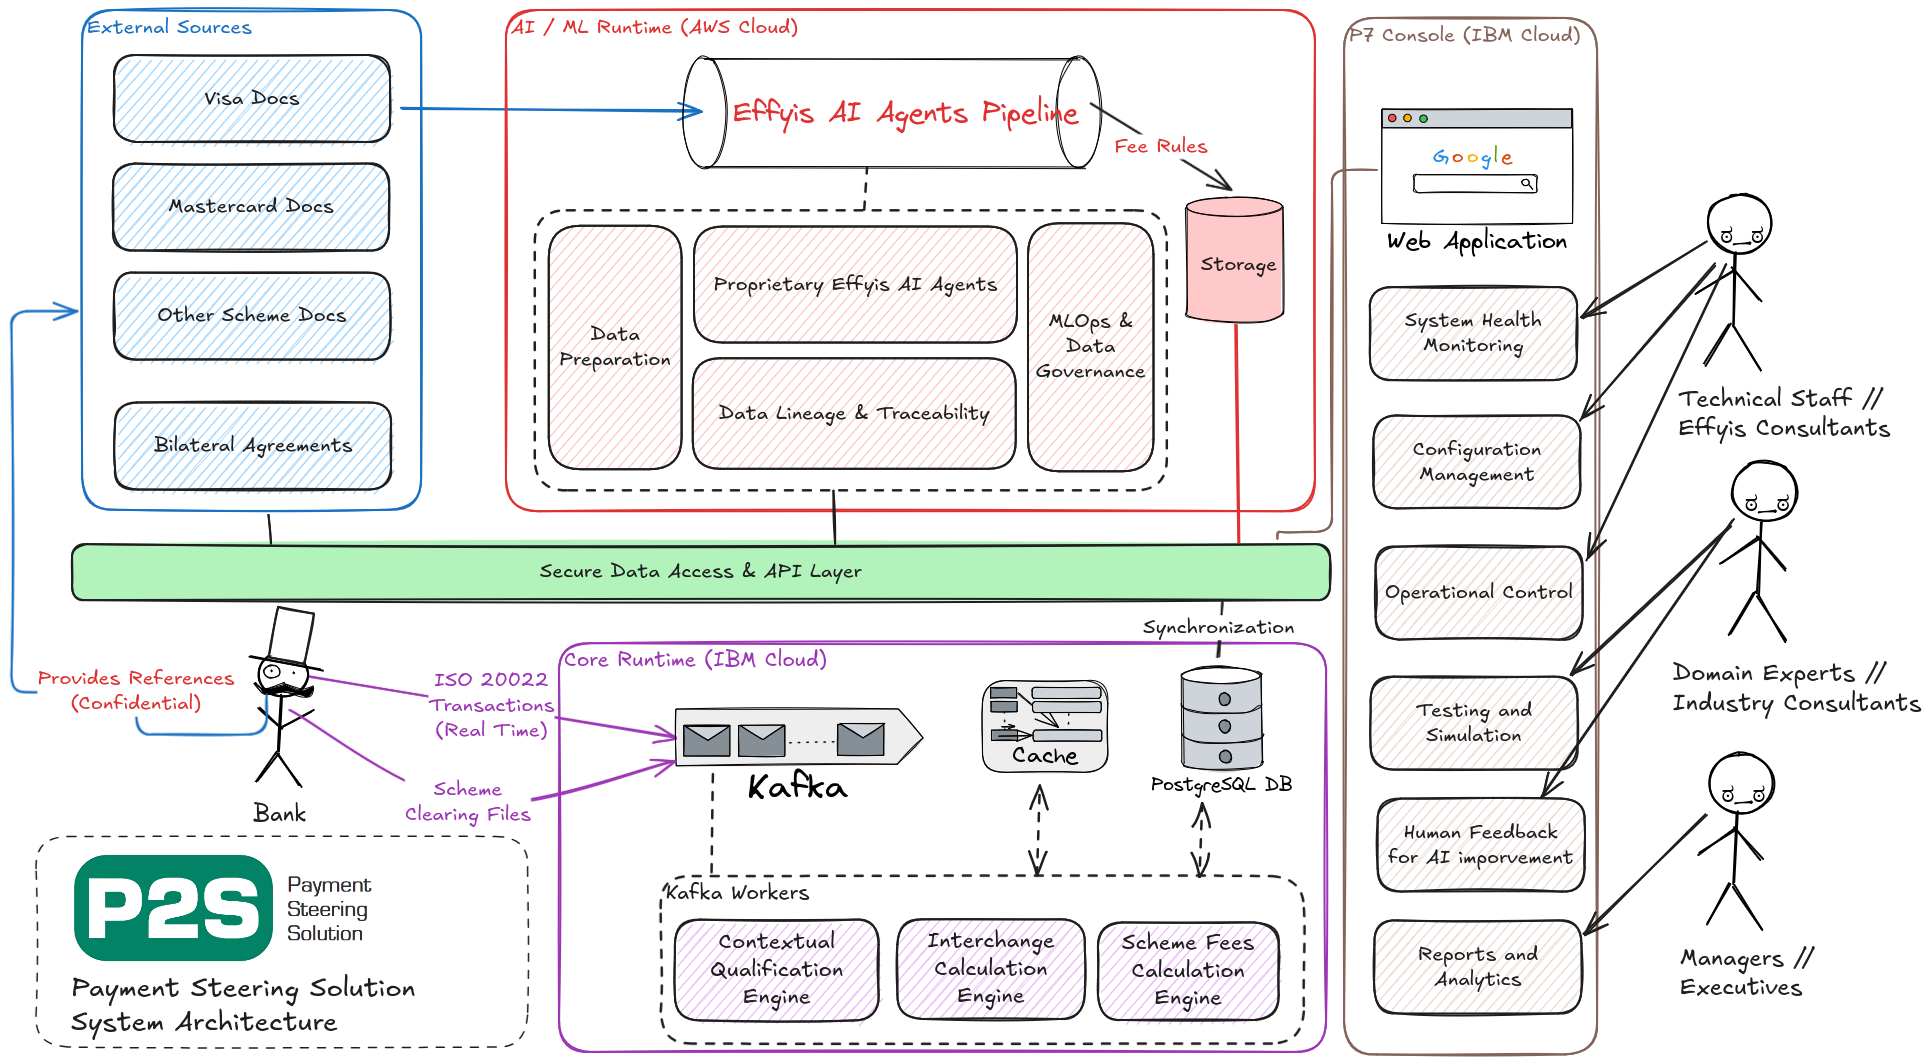
\includegraphics[width=\textwidth]{img/arch/new_archi.png}
    \caption{P2S Ecosystem Architecture Overview}
    \label{fig:solution_architecture}
\end{figure}

The ecosystem architecture, illustrated in Figure~\ref{fig:solution_architecture}, demonstrates the integration between document processing capabilities and real-time transaction processing infrastructure. This separation of concerns enables specialized optimization of each component while maintaining seamless data flow and operational coherence throughout the system.

\subsection{AI Agents Pipeline Integration}

The P2S compute engines rely on structured data extracted and normalized by the AI Agents Pipeline, which serves as the document understanding foundation of the ecosystem. This pipeline transforms unstructured payment scheme documentation from various financial institutions into standardized, machine-readable rule sets that feed directly into the compute engines.

\begin{figure}[H]
    \centering
    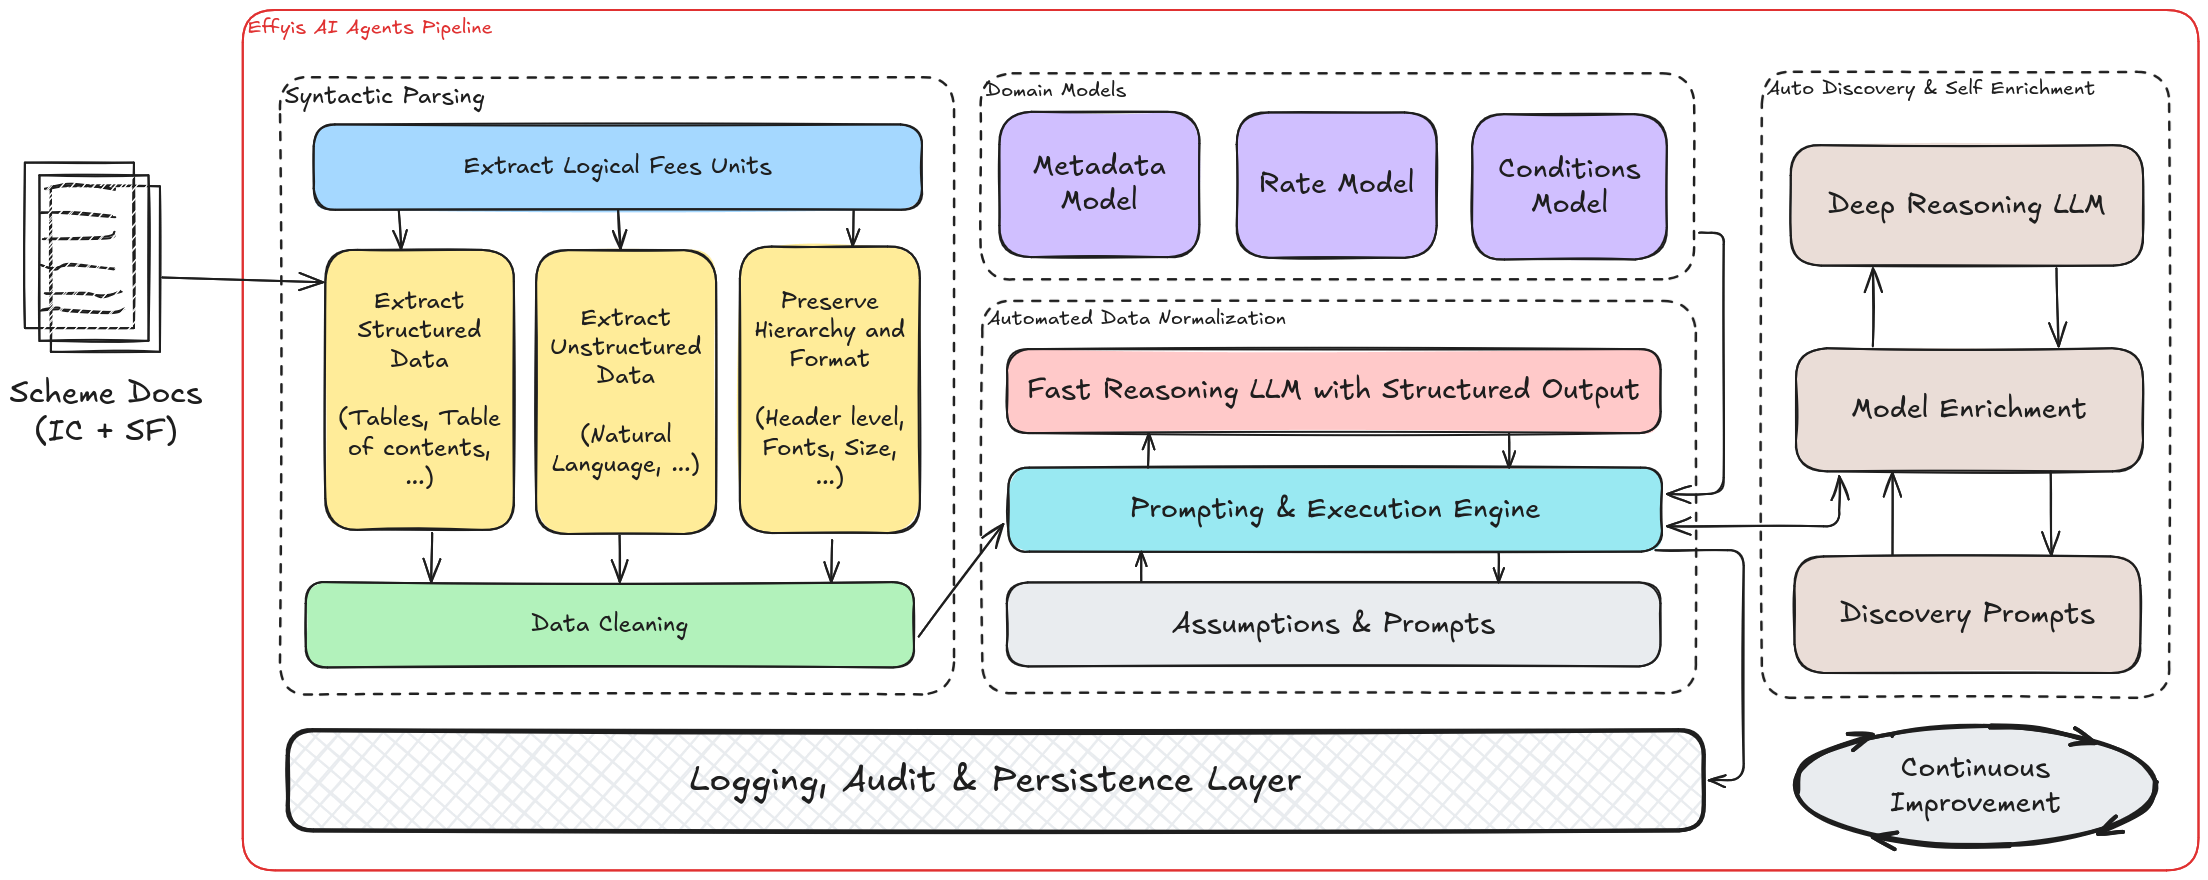
\includegraphics[width=\textwidth]{img/arch/pipeline_design.png}
    \caption{AI Agents Pipeline - Data Source for Compute Engines}
    \label{fig:ai_pipeline_architecture}
\end{figure}

The AI pipeline outputs normalized fee structures, qualification rules, and rate tables that are essential for the compute engines' operation. This preprocessing ensures that the real-time processing engines can focus on high-performance transaction processing without the computational overhead of document interpretation during runtime.

Key outputs from the AI pipeline that feed into the compute engines include:
\begin{itemize}
    \item Structured interchange fee matrices with qualification criteria
    \item Normalized scheme fee tables with applicable rate structures  
    \item Contextual qualification rules for transaction categorization
    \item Cost code mappings and hierarchical fee structures
\end{itemize}

\subsection{P2S Compute Engines Architecture}

This section presents the core architecture of the P2S compute engines, which constitute the primary focus of this thesis. The compute engines implement a distributed, event-driven architecture specifically designed for high-throughput, real-time fee calculation processing.

\subsubsection{Architectural Design Principles}

The P2S compute engines architecture is founded on several key design principles that enable scalable, reliable, and maintainable transaction processing:

\textbf{Stateless Processing}: All compute engines operate as stateless components, enabling horizontal scaling and eliminating single points of failure. State management is externalized through caching layers and persistent storage systems.

\textbf{Event-Driven Communication}: The architecture leverages Apache Kafka as the primary communication backbone, enabling asynchronous, fault-tolerant message processing with built-in durability and replay capabilities.

\textbf{Microservices Separation}: Each processing concern is isolated into dedicated microservices, allowing independent development, deployment, and scaling of individual components.

\textbf{Fail-Fast Error Handling}: Comprehensive error handling with dedicated error channels ensures system resilience while maintaining operational visibility.

\subsubsection{Core Compute Engine Components}

The P2S compute engines consist of four specialized processing components, each responsible for specific aspects of transaction fee calculation:

\begin{figure}[H]
    \centering
    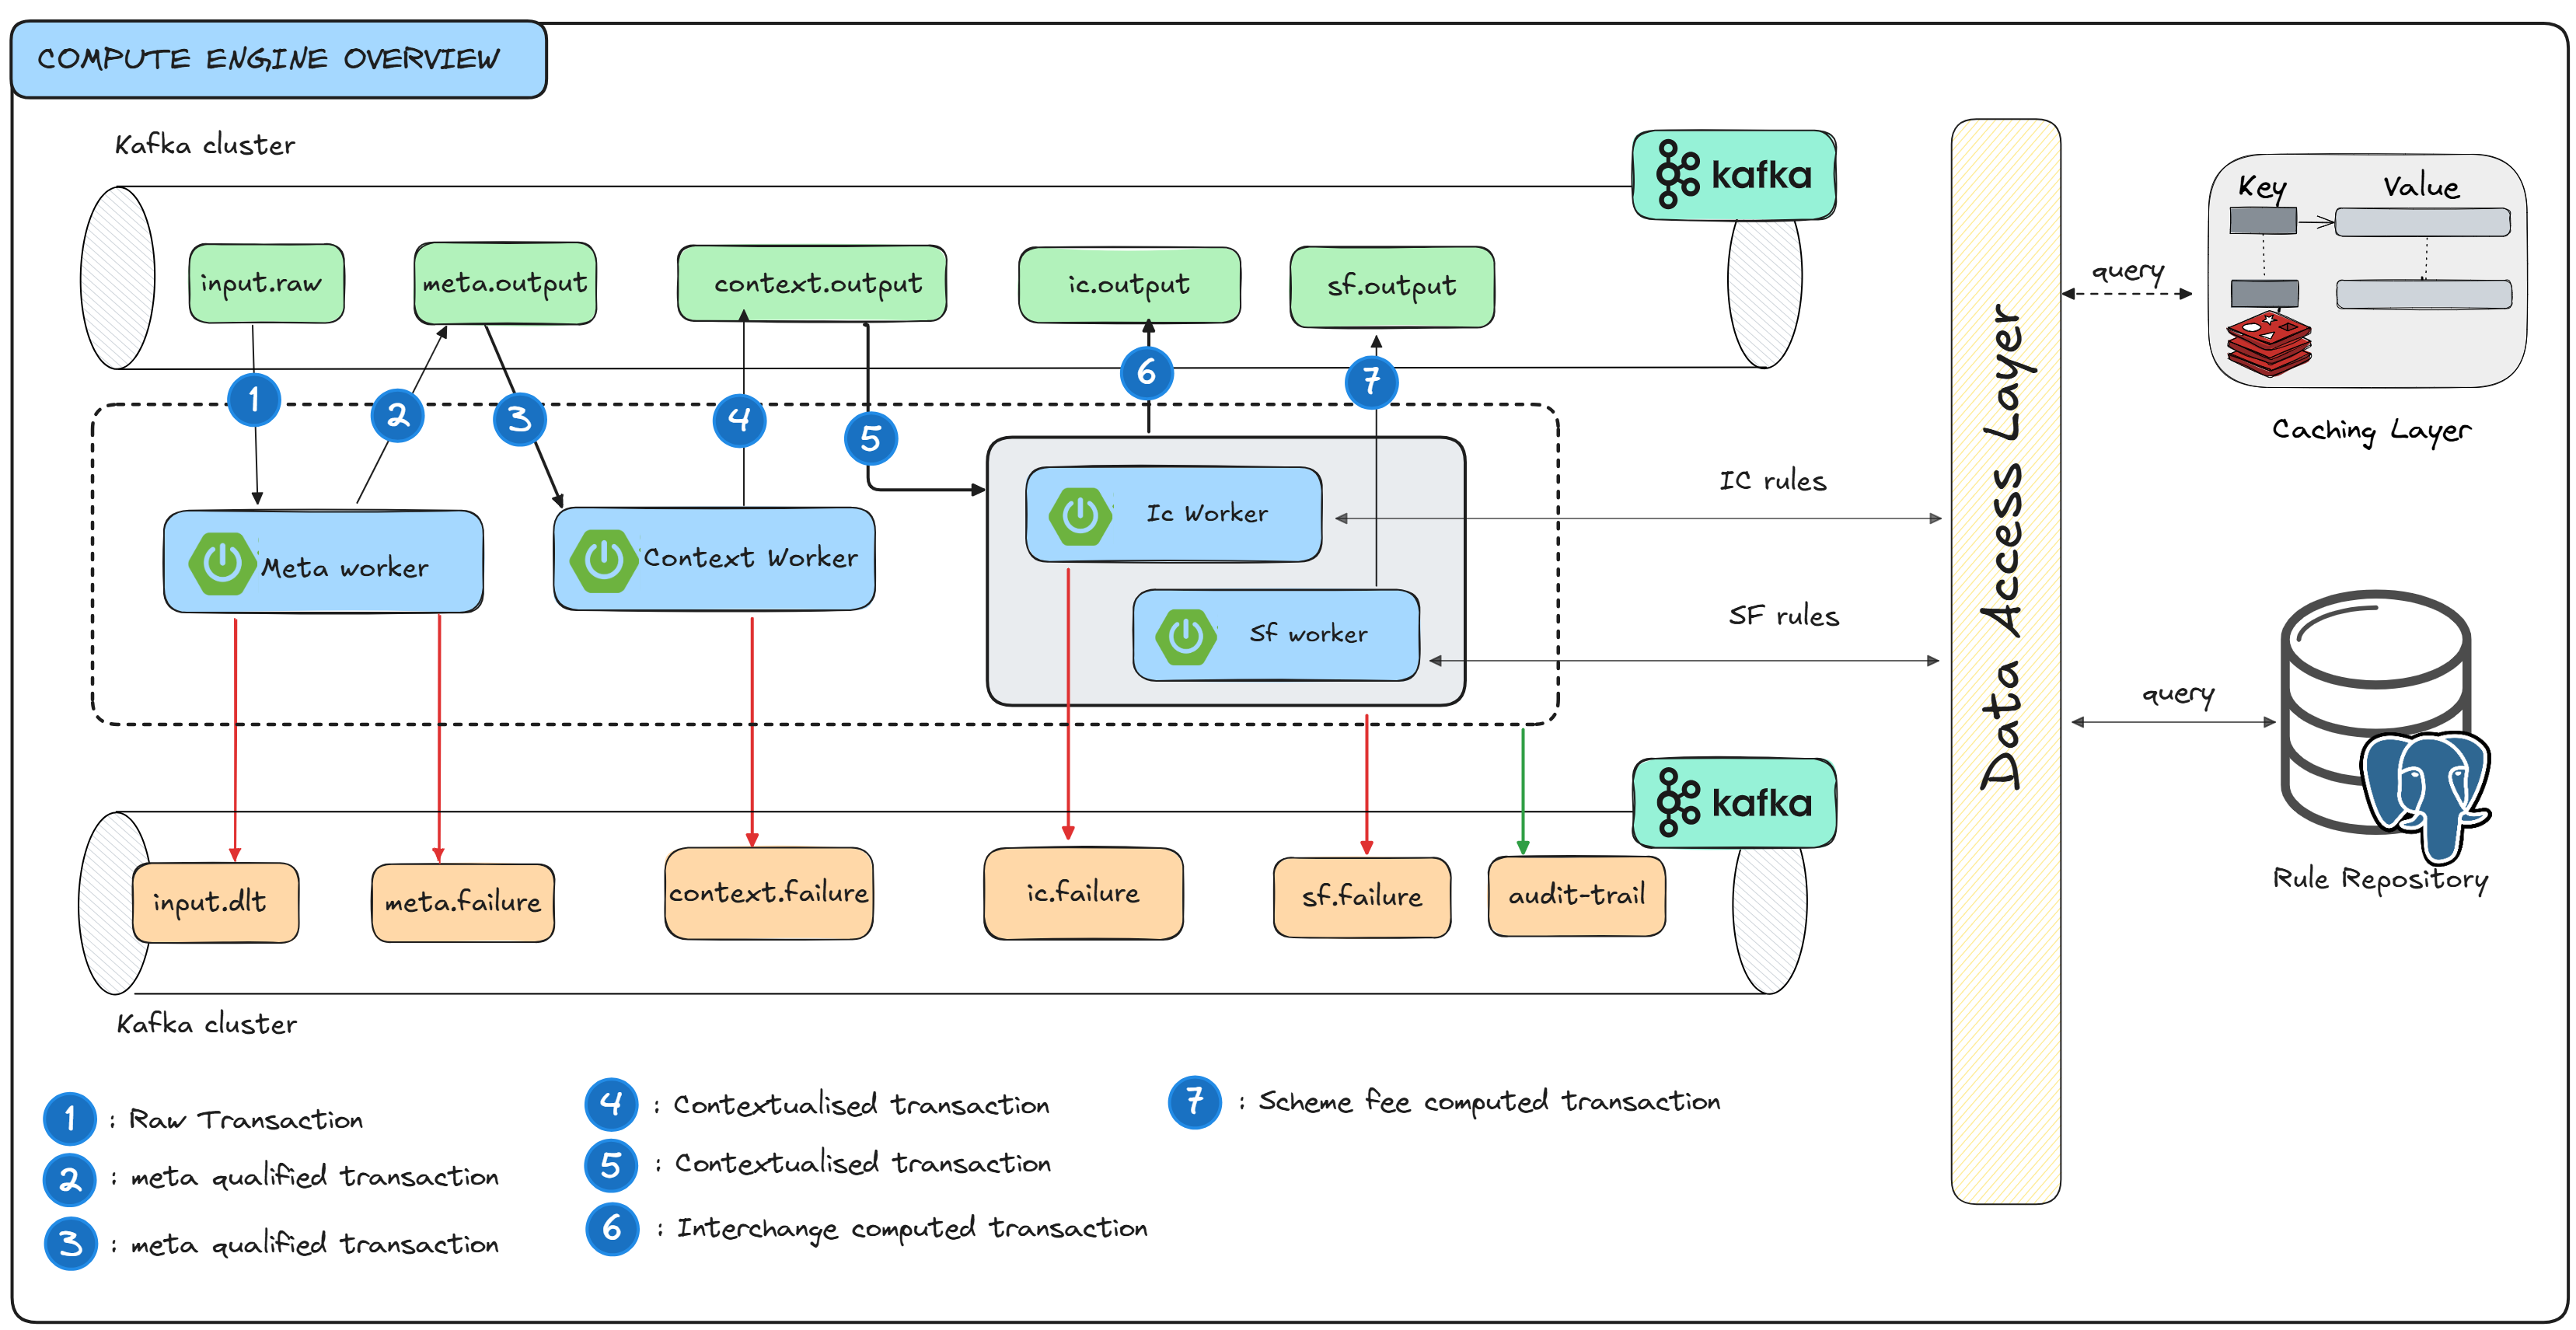
\includegraphics[width=1\textwidth]{img/arch/stateless-architecture.png}
    \caption{P2S Compute Engines Detailed Architecture}
    \label{fig:compute_engines_architecture}
\end{figure}

\textbf{Meta Worker Engine}

The Meta Worker serves as the intelligent transaction dispatcher and initial processing coordinator. This component receives raw transaction data from input topics and performs critical preprocessing tasks:

\begin{itemize}
    \item Transaction validation and format standardization
    \item Bank Identification Number (BIN) resolution and geographical classification
    \item Payment scheme identification and routing decision logic
    \item Initial transaction enrichment with metadata attributes
    \item Intelligent load distribution across downstream processing engines
\end{itemize}

The Meta Worker implements sophisticated routing algorithms that analyze transaction characteristics to determine optimal processing pathways, thereby minimizing latency and maximizing throughput efficiency.

\textbf{Context Qualification Engine}

The Context Qualification Engine performs comprehensive analysis of transactional context to determine applicable fee calculation scenarios. This engine evaluates multiple contextual dimensions:

\begin{itemize}
    \item Issuer and acquirer geographical jurisdictions and regulatory frameworks
    \item Currency conversion requirements and Dynamic Currency Conversion (DCC) status
    \item Card product classification and premium service indicators
    \item Transaction channel and authentication method analysis
    \item Merchant category classification and risk assessment parameters
\end{itemize}

The engine applies complex qualification rules derived from the AI pipeline's normalized documentation to categorize transactions into appropriate fee calculation contexts.

\textbf{Interchange Calculation Engine}

The Interchange Calculation Engine implements sophisticated algorithms for computing interchange fees based on bilateral agreements and payment scheme regulations. Key capabilities include:

\begin{itemize}
    \item Multi-dimensional fee matrix evaluation based on transaction attributes
    \item Regulatory compliance validation for interchange fee caps and regulations
    \item Bilateral agreement application with priority-based rule resolution
    \item Volume-based fee calculation with progressive rate structures
    \item Cross-border transaction handling with currency conversion considerations
\end{itemize}

This engine maintains high performance through optimized rule evaluation algorithms and caching strategies for frequently accessed fee structures.

\textbf{Scheme Fees Calculation Engine}

The Scheme Fees Calculation Engine processes payment scheme-specific fees according to proprietary methodologies established by individual payment networks. Capabilities encompass:

\begin{itemize}
    \item Cost code resolution and hierarchical fee structure application
    \item Volume threshold management with progressive pricing models
    \item Special service fee calculation for premium transaction types
    \item Scheme-specific promotion and discount application logic
    \item Regulatory fee computation for compliance-related charges
\end{itemize}

The engine implements flexible rule evaluation frameworks that can accommodate diverse payment scheme methodologies while maintaining consistent performance characteristics.

\subsubsection{Data Flow and Processing Pipeline}

The P2S compute engines implement a sophisticated data flow architecture that ensures reliable, traceable, and efficient transaction processing:

\textbf{Input Processing Flow}:
\begin{enumerate}
    \item Raw transaction data enters via the \texttt{input-raw} Kafka topic
    \item Meta Worker performs initial processing and enrichment
    \item Enriched transactions flow to \texttt{meta-output} topic for downstream consumption
    \item Error conditions are captured in dedicated \texttt{meta-errors} topic
\end{enumerate}

\textbf{Context Processing Flow}:
\begin{enumerate}
    \item Context Qualification Engine consumes from \texttt{meta-output} topic
    \item Contextual analysis and qualification rule application
    \item Qualified transactions published to \texttt{p2s-context-out} topic
    \item Context-related errors captured in \texttt{p2s-context-errors} topic
\end{enumerate}

\textbf{Fee Calculation Flow}:
\begin{enumerate}
    \item Both Interchange and Scheme Fee engines consume from \texttt{p2s-context-out}
    \item Parallel processing enables simultaneous fee calculation
    \item Interchange results published to \texttt{p2s-ic-out} topic
    \item Scheme fee results published to \texttt{p2s-sf-out} topic
    \item Respective error topics capture processing exceptions
\end{enumerate}

\textbf{Audit and Monitoring}:
\begin{enumerate}
    \item Comprehensive audit trail captured in \texttt{p2s-audit} topic
    \item Real-time monitoring through dedicated observability infrastructure
    \item Error aggregation and alerting for operational visibility
\end{enumerate}

\subsubsection{Scalability and Performance Architecture}

The compute engines architecture incorporates several design elements specifically engineered for high-performance, scalable operation:

\textbf{Horizontal Scaling}: Each engine operates as independent Kafka consumers that can be scaled horizontally by increasing consumer group membership. This approach enables linear scaling with transaction volume growth.

\textbf{Partitioning Strategy}: Kafka topic partitioning is optimized based on transaction routing keys to ensure balanced load distribution while maintaining processing order where required.

\textbf{Caching Architecture}: Multi-tier caching implementation reduces database load and improves response times for frequently accessed fee structures and qualification rules.

\textbf{Circuit Breaker Pattern}: Integrated circuit breakers prevent cascade failures and enable graceful degradation during high-load or error conditions.

\textbf{Asynchronous Processing}: Non-blocking, asynchronous processing patterns maximize resource utilization and system throughput.

\subsubsection{Reliability and Error Handling}

The architecture implements comprehensive reliability mechanisms to ensure consistent operation in production environments:

\textbf{Fault Isolation}: Component failures are isolated through dedicated error channels and do not impact other processing components.

\textbf{Retry Mechanisms}: Configurable retry policies with exponential backoff handle transient failures automatically.

\textbf{Dead Letter Queues}: Persistent error handling through dedicated dead letter topics ensures no transaction loss during error conditions.

\textbf{Health Monitoring}: Continuous health checks and metrics collection enable proactive identification of performance degradation or failure conditions.

This architecture provides the foundation for reliable, scalable, and maintainable real-time fee calculation processing within the P2S ecosystem, enabling financial institutions to efficiently process high-volume transaction flows while maintaining accuracy and compliance requirements.







\section{Technical Stack}

\subsection{Core Development Platform}

\textbf{Java:} Primary programming language providing platform independence, strong type system, and extensive ecosystem for enterprise application development.

\textbf{Spring Boot:} Application framework enabling rapid development of microservices with auto-configuration, embedded servers, and production-ready features.

\subsection{Data Management}

\textbf{PostgreSQL:} Primary relational database for transactional data storage, providing ACID compliance and complex query support.

\textbf{Redis:} In-memory caching solution for frequently accessed data, reducing database load and improving response times.

\subsection{Event Processing}

\textbf{Apache Kafka:} Distributed event streaming platform for real-time data pipeline management and inter-service communication.

\textbf{Apache Avro:} Data serialization framework ensuring efficient data exchange and schema evolution capabilities.

\textbf{Confluent Schema Registry:} Centralized schema management for Kafka topics, ensuring data consistency across microservices.

\subsection{Development Operations}

\textbf{GitLab:} Source code management and CI/CD pipeline automation for collaborative development and deployment.

\textbf{Docker:} Containerization platform ensuring consistent deployment environments and horizontal scaling capabilities.

\textbf{Apache Maven:} Build automation and dependency management for Java projects.

\section{Chapter Conclusion}

This chapter has established the comprehensive foundation for the \textbf{proof-of-concept stateless computational architecture} development within the P2S financial platform. The analysis reveals significant challenges in contemporary payment processing systems, particularly in structural representation of fee rules and computational efficiency in their application.

The identified problems - heterogeneous documentation formats and computational bottlenecks - directly impact operational efficiency and cost structures for financial institutions. The proposed proof-of-concept addresses these challenges through demonstrating the viability of stateless computational engines that can form the foundation for future production-scale implementation.

Effyis Group provides an ideal environment for this proof-of-concept development, with its specialized focus on payment systems and established P2S platform infrastructure. The company's flat organizational structure and agile development practices support the iterative approach necessary for validating complex financial system architectures.

The adoption of Scrum methodology ensures structured project management while maintaining flexibility for technical experimentation and validation. The comprehensive technical stack, centered on Java and Spring Boot with supporting technologies for data management and event processing, provides a robust foundation for implementing and testing the proposed architectural concepts.

\textbf{Project Positioning:} This internship project serves as a critical foundation phase, developing and validating core architectural concepts that will guide the subsequent production-scale implementation of the complete P2S fee calculation system. The proof-of-concept approach allows for thorough validation of technical assumptions and performance characteristics before committing to full-scale production development.

The next chapter will provide detailed analysis of the payment industry domain, establishing the business and technical context necessary for understanding the computational challenges that motivate the architectural approach validated in this proof-of-concept implementation.
